\chapter{Зависимость насыщающего вейбелевскую неустойчивость магнитного поля от вида распределения частиц по скоростям в одномерном и двумерном случаях}
\newcommand{\PunctumKappa}{-}
\label{ch:ch5}
Ниже зависимость насыщающего магнитного поля вейбелевской турбулентности от начальной анизотропии частиц исследуется для бикаппа{\PunctumKappa}распределения~\cite{Vasyliunas1968, Lazar2010, Livadiotis2017, Livadiotis2021, Pierrard2010}. Оно свойственно неравновесной плазме, частицы которой испытали стохастическое ускорение под действием того или иного широкополосного электромагнитного излучения, например в звездном ветре или различных ударных волнах, и в качестве частного случая содержит бимаксвелловское распределение частиц по скоростям. 

Для определенности эффективная температура частиц считается наибольшей вдоль оси $y$. Тогда если бы в трехмерном случае функция распределения (ФР) частиц обладала аксиальной симметрией по отношению к скоростям в плоскости $x,z$, то неустойчивость развивалась только для волновых возмущений необыкновенного типа и приводила к ТМ-вейбелевской турбулентности~\cite{Kalman1968, Vagin2014}. Имея в виду аналогичную ситуацию для рассматриваемых ниже двумерных расчетов, будем считать ФР симметричной по проекции скорости частиц на ось $x$, т.\,е. не зависящей от знака этой проекции. Для интересующих нас ТМ-возмущений волновые векторы гармоник электромагнитного поля и соответствующих гармоник анизотропной ФР энергонесущих частиц (пусть электронов), как и вектор электрического поля, лежат в плоскости $x,y$, а вектор магнитного поля ортогонален этой плоскости, т.\,е. параллелен оси $z$ (рис.~\ref{fig:GeomIsolines}б). Неустойчивость насыщается, т.\,е. прекращается рост среднеквадратичного магнитного поля, тогда, когда оно в достаточной мере выравнивает средние значения продольной ($T_{\|}$, вдоль оси $y$) и поперечной ($T_\perp $, вдоль оси $x$) эффективных температур. При этом присутствие этого поля, его пространственная неоднородность и понизившийся и тоже неоднородный уровень анизотропии $A=T_{\|} / T_{\perp} - 1$ исключают экспоненциальное нарастание каких-либо возмущений, в том числе крупномасштабных, хотя слабонелинейная перестройка пространственного спектра турбулентности в длинноволновую сторону продолжается и далее (см.,~например,~\cite{Kocharovsky2016,Zhou2022, Borodachev2016_Radiofiz,Dieckmann2009,Romanov2004}).
\begin{figure}[h]
\begin{minipage}[c]{0.5\linewidth}
    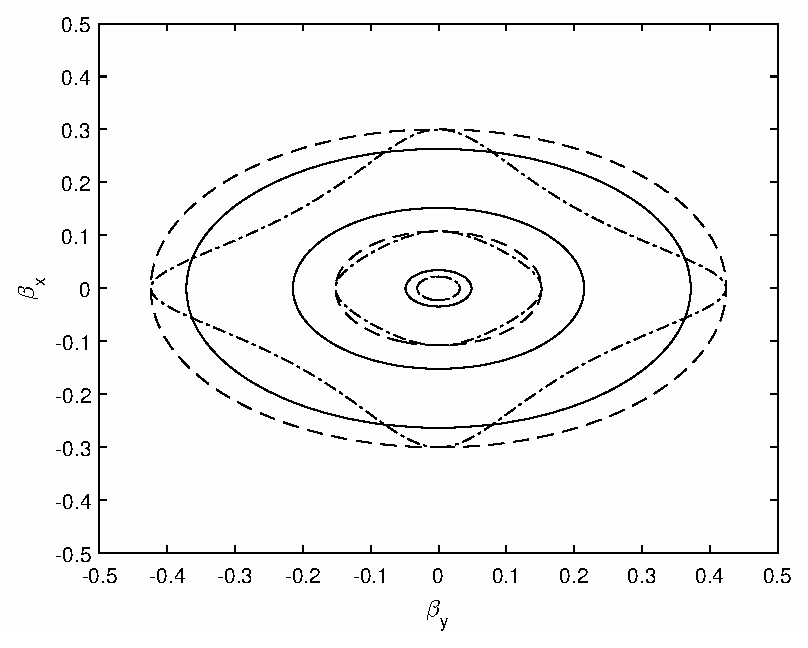
\includegraphics[width=1\linewidth]{part5/levels.eps}
\end{minipage}
\begin{minipage}[c]{0.5\linewidth}
    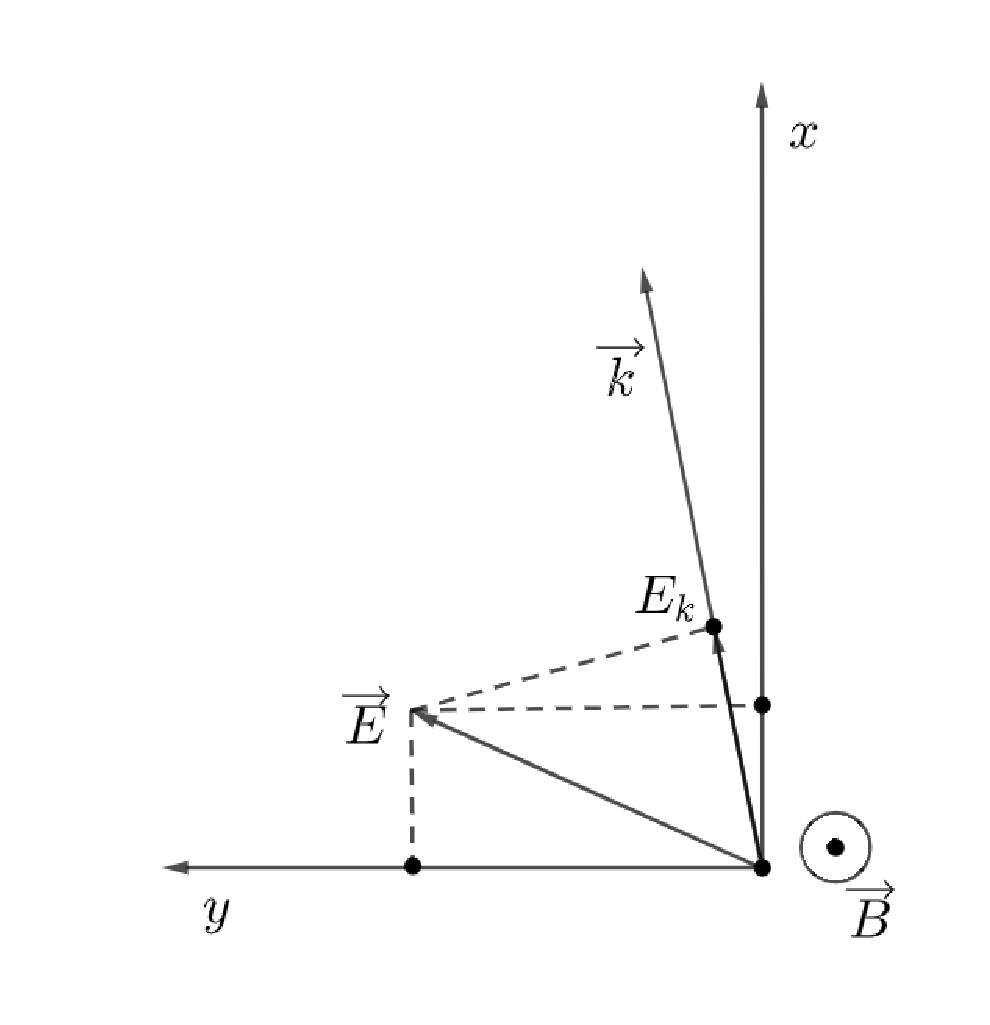
\includegraphics[width=1\linewidth]{part5/new_image.eps}
\end{minipage}
\captionstyle{normal}
    \caption{
    а)~Линии уровня $0.001$, $0.1$ и $0.9$ от максимального значения для бимаксвелловской (сплошная кривая), бикаппа{\PunctumKappa} (штриховая) и продакт-бикаппа{\PunctumKappa} (штрихпунктир) функций распределения электронов по нормированным скоростям $\beta_x$ и $\beta_y$ при $\kappa=2$, поперечной (вдоль оси~$x$) тепловой скорости $\beta_\perp=0.1$ и параметре анизотропии $A = 1$. 
    б)~Взаимное расположение волнового вектора $\vec{k}$, лежащего в плоскости $x,y$, и векторов магнитного $\vec{B}$ и электрического $\vec{E}$ полей в отдельной пространственной гармонике ТМ-вейбелевской турбулентности.
    }
\label{fig:GeomIsolines}
\end{figure}
Детальнее постановка задачи, используемые приближения, схема вывода уравнений и особенности расчетов даны в следующем разделе. Далее приведены основные результаты расчетов, касающиеся зависимости насыщающего магнитного поля вейбелевской турбулентности от начальной анизотропии плазмы и от основного параметра $\kappa$ энергетического каппа{\PunctumKappa}распределения. В заключительном разделе полученные выводы соотнесены с рядом актуальных проблем физики космической и лазерной плазмы. Проведенное моделирование показало также богатую динамику пространственного спектра вейбелевской турбулентности и согласованной деформации функции распределения частиц на долговременной нелинейной стадии неустойчивости после ее насыщения. Однако изложение результатов такого рода выходит за рамки настоящего краткого сообщения и будет дано в более подробной статье. 

\section{Постановка задачи, уравнения для гармоник и схема их решения}

Для бесстолкновительной плазмы, в которой на рассматриваемых временах насыщения неустойчивости можно пренебречь движением тяжелых ионов, самосогласованные уравнения Власова~-- Максвелла для функции распределения электронов $f(v_x , v_y , x, y, t)$, включающей их концентрацию $N (x, y, t)$, и электрического $\vec{E}=(E_x, E_y, 0)$ и магнитного $\vec{B}=(0, 0, B_z)$ полей имеют вид
\begin{eqnarray}
    \dfrac{\partial f}{\partial t}+\vec{v}\dfrac{\partial f}{\partial \vec{r}}+\dfrac{e}{\me} \left(\vec{E}+\dfrac{1}{c}\left[\vec{v},\vec{B}\right]\right) \dfrac{\partial f}{\partial \vec{v}}=0, \\
    %
    \label{eq:maxw1} 
    \nabla \times \vec{B}=\dfrac{1}{c}\dfrac{\partial \vec{E}}{\partial t}+\dfrac{4\pi}{c}\vec{j}, \\
    %
    \label{eq:maxw2}
    \nabla \times \vec{E}=-\dfrac{1}{c}\dfrac{\partial \vec{B}}{\partial t},
\end{eqnarray}
где $c$~--- скорость света в вакууме, $e$ и $\me$~--- заряд и масса электрона, $\vec{j}=e\iint^{+\infty}_{-\infty}\vec{v}f(v_x , v_y , x, y, t) dv_x dv_y$~--- плотность тока, $N=\iint^{+\infty}_{-\infty}f(v_x , v_y , x, y, t)dv_xdv_y$ и учтено, что векторы координаты и скорости имеют только две компоненты, $\vec{r}=(x , y ,0)$ и $\vec{v}=(v_x , v_y ,0)$, согласно двумерной постановке задачи. 

Предположим, что в начальный момент времени нормированная на единицу функция распределения имеет вид бикаппа{\PunctumKappa}распределения с $\kappa >  1$, 
\begin{equation}
\label{eq:kappa}
    \Psi(\vec{\beta})=\dfrac{1}{\pi\theta_{\perp}\theta_{\|} } \left(1+\dfrac{\beta_x^2}{\kappa\theta_{\perp}^2}+\dfrac{\beta_y^2}{\kappa\theta_{\|}^2}\right)^{-\kappa-1} ,
\end{equation}
либо продакт-бикаппа{\PunctumKappa}распределения с $\kappa > 1/2$, 
\begin{equation}
\label{productkappa}
\Psi(\vec{\beta}) = \dfrac{\Gamma^2(\kappa+1)}{\Gamma^2(\kappa+0.5)} \: \dfrac{1}{\pi\kappa\theta_{\perp}\theta_{\|}}\left(1+\dfrac{\beta_x^2}{\kappa\theta_{\perp}^2}\right)^{-\kappa-1} \!\left(1+\dfrac{\beta_y^2}{\kappa\theta_{\|}^2}\right)^{-\kappa-1};
\end{equation}
см.~\cite{Lazar2010, Livadiotis2017, Livadiotis2021,Pierrard2010}. Выше $\beta_{x,y}={v_{x,y}}/{c}$, т.\,е. $\vec{\beta}=\vec{v}/{c}$, и введены характерные скорости $\theta_{\perp,\|}=\beta_{\perp,\|}\left(1-1/\kappa\right)^{1/2}$ для бикаппа{\PunctumKappa}распределения и $\theta_{\perp,\|}=\beta_{\perp,\|}\left(1-1/(2\kappa)\right)^{1/2}$ для продакт-бикаппа{\PunctumKappa}распределения с использованием эффективных тепловых скоростей $\beta_{\perp,\|}={v_{T_{x,y}}}/{c}$ вдоль осей $x$ и $y$ соответственно, так что параметр анизотропии
\begin{equation}
A={\beta^2_{\|}}/{\beta^2_{\perp}}-1={\theta^2_{\|}}/{\theta^2_{\perp}}-1.
\end{equation}

В пределе $\kappa \rightarrow \infty$ распределения (\ref{eq:kappa}), (\ref{productkappa}) сводятся к бимаксвеллловскому:
\begin{equation}
\label{bimax}
\Psi(\vec{\beta})=\dfrac{1}{\pi\beta_{\perp} \beta_{\|} } \exp\left(-\dfrac{\beta_x^2}{\beta_{\perp}^2}-\dfrac{\beta_y^2}{\beta_{\|}^2}\right).
\end{equation}
Его характерные сечения, как и сечения распределений (\ref{eq:kappa}), (\ref{productkappa}) при $\kappa=2$, представлены на рис.~\ref{fig:GeomIsolines}а для параметра анизотропии $A=1$. Здесь и ниже в иллюстрациях и расчетах для определенности полагаем $\beta_{\perp}=0.1$: конкретное значение этого параметра не влияет на основные выводы работы. На рис.~\ref{fig:GeomIsolines}б для поставленной задачи показано расположение векторов электрического $\vec{E}$ и магнитного $\vec{B}$ полей рассматриваемых однородных гармоник необыкновенного типа $\exp(-i\vec{k}\vec{r})$ с волновым вектором $\vec{k}$, проекция на который электрического поля в общем случае не равна нулю: $E_k\neq0$.

С целью анализа насыщения развивающейся ТМ-вейбелевской неустойчивости используем приближенный метод разложения по пространственным гармоникам решения уравнений Власова~-- Максвелла с шумоподобным начальным возмущением магнитного поля, обладающим примерно равномерным спектром в области неустойчивых волновых чисел. Такой метод можно применять в виду слабой нелинейности (квазилинейности) кинетического уравнения Власова в рассматриваемых условиях: для любой отдельной гармоники магнитного (и соответствующего электрического) поля $B_1(t,\vec{r})= \mathrm{Re} \left[ B_1(t)\exp(-i\vec{k} \vec{r}) \right]$ с волновым вектором $\vec{k}$ можно не учитывать кратные гармоники $\ell \vec{k}$ с целым $\ell > 1$ и необходимо учесть только три гармоники поправок к ФР, $\delta f_\ell(t, \vec{r})=\mathrm{Re} \left[ f_\ell(t)\exp(-i\ell\vec{k}\vec{r}) \right]$, со значениями $\ell =$ 0, 1, 2. При этом наличие большого числа однотипных гармоник, обладающих случайными фазами и достаточно плотно заполняющих значимую область волновых векторов, обеспечивает гладкую форму и плавность изменения ФР, исключая сколько-нибудь значительные эффекты когерентной интерференции и допуская неадекватный вид ФР, например отрицательные ее значения, только при скоростях много больше эффективных тепловых, т.\,е. для очень малой, несущественной фракции электронов.

Применимость теории возмущений, а практически~--- соблюдение иерархии малости амплитуд последующих гармоник по сравнению с предыдущими (как гармоник ФР, $\delta f_ \ell\gg \delta f_{\ell+1}$, так и аналогичных гармоник магнитного или электрического полей) проверено нами в наиболее опасном случае задания лишь одной производящей гармоники с волновым вектором $\vec{k}$, направленным вдоль $\vec{x_0}$, ортогонально оси анизотропии~$y$. В этом случае неустойчивость развивается быстрее всего, а задача фактически становится одномерной, причем нелинейно связываются все кратные гармоники ФР $\ell\vec{k}$ с $\ell =$ 0, 1, 2, 3,~... и лишь нечетные гармоники ТМ-поля $\ell\vec{k}$ с $\ell =$ 1, 3,~... (в силу отсутствия токов на четных гармониках из-за свойств четности ФР). Здесь и ниже $\vec{x_0}$, $\vec{y_0}$, $\vec{z_0}$~--- единичные орты декартовой системы координат.

Следуя теории возмущений до $\ell = 3$ и опуская очевидные осцилляторные уравнения для первой и третьей гармоник магнитного поля,
\begin{equation}
    \vec{B} = \mathrm{Re} \left[ B_1(t) \exp(-ikx)+B_3(t)\exp(-3ikx) \right] \vec{z_0} ,
\end{equation}
получающиеся из уравнений (\ref{eq:maxw1}), (\ref{eq:maxw2}) и в силу их линейности включающие только соответствующие первую и третью гармоники ФР, нетрудно прийти к следующей системе связанных уравнений для кратных (комплексных) гармоник-возмущений ФР:
\begin{equation}
    \dfrac{\partial f_0}{\partial t}+\hat \phi(\Omega_1,f_1^*)+\hat \phi^*(\Omega_1^*,f_1)=0 ,
\label{eq6}
\end{equation}
\begin{equation}
    \dfrac{\partial f_1}{\partial t}+ikv_xf_1+2\hat \phi(\Omega_1,F(\vec{v})+f_0)+\hat \phi^*(\Omega_1^*,f_2)=0 ,
\label{eq7}
\end{equation}
\begin{equation}
    \dfrac{\partial f_2}{\partial t}+2ikv_xf_2+\hat \phi(\Omega_1,f_1)=0 ,
\label{eq8}
\end{equation}
\begin{equation}
    \dfrac{\partial f_3}{\partial t}+3ikv_xf_3+2\hat \phi(\Omega_3,F(\vec{v}))+\hat \phi(\Omega_1,f_2)=0 .
\label{eq9}
\end{equation}
Для сокращения записи введены оператор
\begin{equation}
    \hat \phi(\Omega_{1},f(\vec{v}))=\dfrac{i}{2k}\dfrac{\partial\Omega_{1}}{\partial t} \dfrac{\partial f(\vec{v})}{\partial v_y}-\dfrac{1}{2}\Omega_{1} \left(v_x\dfrac{\partial f(\vec{v})}{\partial v_y}-v_y\dfrac{\partial f(\vec{v})}{\partial v_x}\right) 
\label{eq12}
\end{equation}
и комплексная гирочастота $\Omega_1={e B_1}/{(\me c)}$. Качественные оценки и численные решения полученной системы уравнений показывают, что насыщение отдельной основной гармоники магнитного поля $B_1(t)$, непосредственно создаваемой первой гармоникой ФР $f_1(t)$, по существу определяется согласованной динамикой нулевой и второй гармоник ФР $f_0,_2(t)$, но не третьей (и высшими) гармониками магнитного поля и ФР. Благодаря слабой нелинейности (квазилинейности) процесса вейбелевской неустойчивости нарушение применимости используемой теории возмущений можно ожидать лишь для сильно изрезанных анизотропных функций распределения частиц, не представляющих интереса для рассматриваемого нами круга задач.


Используем последнее обстоятельство и в общем случае двумерно-неоднородной задачи с большим числом $m \cdot s$ неколлинеарных производящих гармоник
$\{ (k_{1}; k_{1}),\,\\ (k_{1}; k_{2}),...,\, (k_{2}; k_{1}),...\, (k_{m}; k_{s}) \}$ (их компоненты состоят из $m$ проекций $\vec{k}\vec{x_0}$ и $s$ проекций $\vec{k}\vec{y_0}$), расположенных часто и перекрывающих всю существенную область волновых векторов неустойчивости. В этом представлении магнитное поле имеет вид суммы по целочисленному векторному индексу $\vec{n}=(n_x,n_y)$:
$B(t,x,y)= \mathrm{Re} \, \sum^{m}_{n_x=1}\sum_{n_y=1}^sB_{k_{\vec{n}}}(t)\exp(- ik_{n_{x}}x - ik_{n_{y}}y)$.
Аналогичный вид имеет каждая из двух кратных гармоник-возмущений ФР, т.\,е. компонент $\delta f_1(t,x,y)$ и $\delta f_2(t,x,y)$, разложенных на комплексные гармоники ${f_1}_{k_{\vec{n}}}(t)$ и ${f_2}_{k_{\vec{n}}}(t)$ соответственно; нулевая (действительная) гармоника $f_0(t)=\delta f_0(t)$ зависит только от вектора скорости и дает поправку к ФР, усредненную по плоскости $x,y$. Подобно обоснованному выше пренебрежению кратными коллинеарными гармониками, в приведенной ниже приближенной системе самосогласованных уравнений исключены неколлинеарные суммарные и разностные гармоники $\vec{k}_j+\vec{k}_i$, $\vec{k}_j-\vec{k}_i$, а также неколлинеарные гармоники вида $2\vec{k}_i\pm\vec{k}_j$:

\begin{equation}
\label{eq14}
    \dfrac{\partial \psi_0}{\partial \tau} 
    + \sum\limits^{m,s}_{n_x,n_y=1}\left( \hat \Phi(b_{K_{\vec{n}}},\psi_{K_{\vec{n}}}^*) 
    + \hat \Phi^*(b_{K_{\vec{n}}}^*,\psi_{K_{\vec{n}}}) \right)=0,
\end{equation}
\begin{equation}
    \dfrac{\partial \psi_{K_{\vec{n}}}}{\partial \tau}+iK_{n_x}\beta_x\psi_{K_{\vec{n}}}+iK_{n_y}\beta_y\psi_{K_{\vec{n}}}+2\hat \Phi(b_{K_{\vec{n}}},\Psi(\vec{v})+\psi_0)+\hat \Phi^*(b_{K_{\vec{n}}}^*,\psi_{2K_{\vec{n}}})=0,
\end{equation}
\begin{equation}
\label{eq16}
    \dfrac{\partial \psi_{2K_{\vec{n}}}}{\partial \tau}+2iK_{n_x}\beta_x\psi_{2K_{\vec{n}}}+2iK_{n_y}\beta_y\psi_{2K_{\vec{n}}}+\hat \Phi(b_{K_{\vec{n}}},\psi_{K_{\vec{n}}})=0,
\end{equation}
\begin{equation}
    \dfrac{\partial b_{K_{\vec{n}}}}{\partial \tau}=-ie_{y{K_{\vec{n}}}}K_{n_x}+ie_{x{K_{\vec{n}}}}K_{n_y},
\end{equation}
\begin{equation}
    \dfrac{\partial e_{x{K_{\vec{n}}}}}{\partial \tau}=ib_{K_{\vec{n}}}K_{n_y}-\beta_{\|}^{-1}\iint\limits^{+\infty}_{-\infty}\beta_x\psi_{K_{\vec{n}}}(\tau,\beta_x,\beta_y)d\beta_xd\beta_y,
\end{equation}
\begin{equation}
\label{eq19}
    \dfrac{\partial e_{y{K_{\vec{n}}}}}{\partial \tau}=-ib_{K_{\vec{n}}}K_{n_x}+\beta_{\|}^{-1}{\iint\limits^{+\infty}_{-\infty}\beta_y\psi_{K_{\vec{n}}}(\tau,\beta_x,\beta_y)d\beta_xd\beta_y} .
\end{equation}
Здесь использованы безразмерные время и волновое число, 
\begin{equation*}
    \tau=\wpl t, \
    K=\dfrac{kc}{\wpl}; \ 
    \wpl^2=\dfrac{4\pi Ne^2}{\me},
\end{equation*}
а также нормированные (комплексные) гармоники магнитного поля и ФР: 
\begin{equation}
\label{eq19plus1}
    b_{K_{\vec{n}}}=\dfrac{B_{K_{\vec{n}}}}{\sqrt{8\pi N T_{\|}}},\
    T_{\|}=\dfrac{m_ec^2\beta_{\|}^2}{2};\
    \psi_{\ell\cdot K_{\vec{n}}}=\dfrac{c^2f_{\ell\cdot K_{\vec{n}}}}{N},\ 
    \ell=0,\,1,\,2.  
\end{equation}
Комплексные компоненты электрического поля $e_{x{K_{\vec{n}}}}$ и $e_{y{K_{\vec{n}}}}$ (см. рис.~\ref{fig:GeomIsolines}б) нормированы так же, как магнитное поле $b_{K_{\vec{n}}}$. Для двумерной задачи введен оператор 
\begin{equation}
\label{eq:operator}
    \hat \Phi(b_{K_n},e_{x{K_{\vec{n}}}},e_{y{K_{\vec{n}}}},\psi(\vec{\beta}))=\dfrac{e_{y{K_{\vec{n}}}}}{2}\dfrac{\partial \psi(\vec{\beta})}{\partial \beta_y}+\dfrac{e_{x{K_{\vec{n}}}}}{2}\dfrac{\partial \psi(\vec{\beta})}{\partial \beta_x}-\dfrac{b_{K_n}}{2} \left(\beta_x\dfrac{\partial \psi(\vec{\beta})}{\partial \beta_y}-\beta_y\dfrac{\partial \psi(\vec{\beta})}{\partial \beta_x}\right)
\end{equation}
который отличается от указанного ранее оператора (\ref{eq12}) в одномерной задаче.

Представленная система интегро-дифференциальных уравнений (\ref{eq14})--(\ref{eq19}) с оператором (\ref{eq:operator}) решалась стандартным методом Стёрмера~-- Верле (Leapfrog)~\cite{Birdsall2018}. 

Шаг по времени $d\tau$ составлял малую величину $d\tau\sim 0.05$--$0.5$ в сравнении с наименьшим временным масштабом рассматриваемой обезразмеренной системы уравнений, который определяется собственными длинами волн магнитного поля и тока ($\sim \! {\pi}/{K}$) и имеет порядок единицы. Расчетная сетка для нормированных скоростей $\beta_x$, $\beta_y$ как переменных трех компонент (\ref{eq14})--(\ref{eq16})  анизотропной ФР, разложенных по производящим гармоникам, выбиралась анизотропной с соответствующими шагами $d\beta_x\sim{\beta_{\perp}}/{15}$ и $d\beta_y\sim{\beta_{\|}}/{15}={\beta_{\perp}\sqrt{1+A}}/{15}$. Количество производящих пространственных гармоник $m\cdot s$ в типичных расчетах составляло несколько тысяч и выбиралось из условия независимости (с точностью до нескольких процентов) вычисляемого магнитного поля насыщения неустойчивости от дальнейшего увеличения чисел $m$ и $s$, что обычно имело место начиная с чисел $\sim\! 100$ и $\sim\! 30$ соответственно. 



\section{Особенности насыщения неустойчивости для различных анизотропных распределений электронов}

Основные результаты численного моделирования вейбелевской неустойчивости в двумерной задаче 2D2V суммированы на рис.~\ref{fig:kappa_sat} и \ref{fig:pr_kappa_sat} в представительном интервале параметров начальной анизотропии $0.1\leq A \leq 20$. 
Как и ожидалось, максимальная величина среднего квадрата нормированного магнитного поля $b_{sat}^2 = {({8\pi N T_{\|}})^{-1}} \sum_{\vec{n}} {|B_{K_{\vec{n}}}|^{2}} $, достигаемая в ходе ТМ-неустойчивости и иногда называемая магнетизацией, растет с увеличением величины $A$. При малых значениях $A < 1$ рост оказывается довольно быстрым и зависящим от энергетического распределения электронов. Он теряет эту зависимость и замедляется при $A > 1$, останавливаясь на уровне немного выше 10\% в пределе $A \gg 1$. О последнем свидетельствуют также контрольные расчеты, выполненные для бимаксвелловского распределения с $A = 1$, $10$, $30$ с использованием кода EPOCH~\cite{Arber2015} в 2D3V подходе, т.\,е. методом частиц в ячейках (PIC) с учетом зависимостей всех величин от двух пространственных координат и всех трех компонент скоростей электронов. 
Результаты применения обоих подходов совпадают с точностью порядка 10\%-30\% и подтверждают известную оценку насыщающего магнитного поля, в которой обратный гирорадиус и гирочастота типичных частиц по порядку величины сравниваются соответственно с волновым числом и инкрементом наиболее сильно выросших гармоник поля~\cite{Borodachev2016_Radiofiz, Nechaev2019_Radiophys, Garasev2022_JPP}, что было проверено для всех проведенных расчетов. Предшествующие аналогичные расчеты для отдельных значений параметра анизотропии $A = 24$ и $A = 99$ см. в~\cite{Morse1971, Stockem2009}. 
\begin{figure}[h]

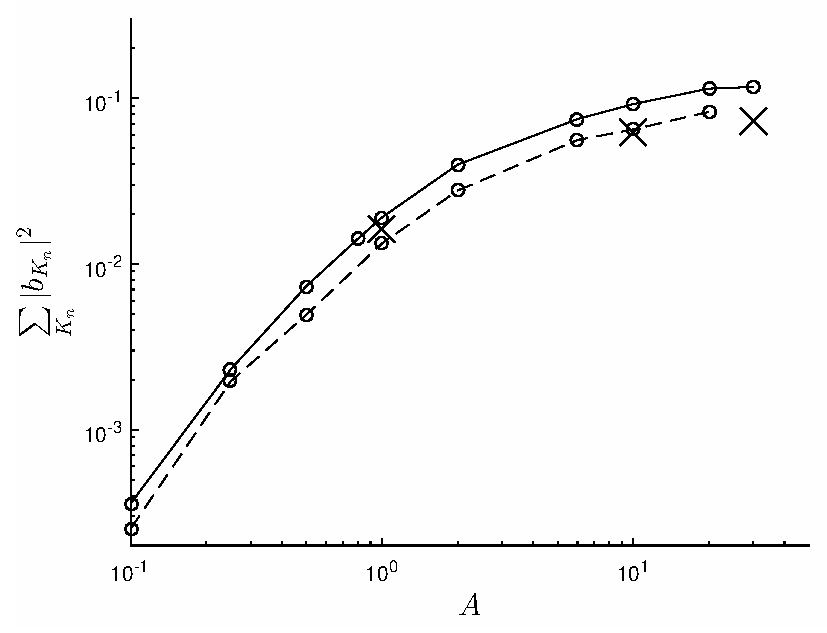
\includegraphics[width=1\linewidth]{part5/14132.eps}
\captionstyle{normal}
\caption{Зависимость среднего квадрата нормированного насыщающего магнитного поля (см. (\ref{eq19plus1}))  от параметра анизотропии $A$ для бикаппа{\PunctumKappa}распределения (\ref{eq:kappa}) при $\beta_\perp=0.1$ и различных значениях параметра каппа:  $\kappa=2$~--- штрихи, $\kappa=\infty$~--- сплошная кривая (бимаксвелловское распределение). В последнем случае крестиками показаны три контрольные точки, рассчитанные в рамках 2D3V кода EPOCH методом частиц в ячейках.}
\label{fig:kappa_sat}
\end{figure}
Осуществленный впервые детальный расчет зависимости насыщающего магнитного поля от параметра анизотропии в данной геометрии задачи стал возможен благодаря разработанному методу на основе уравнений для гармоник (\ref{eq14})--(\ref{eq19}), (\ref{eq:operator}), который позволяет осуществлять вычисления во много раз быстрее, чем метод частиц в ячейках. С использованием последнего трехмерные расчеты подобной зависимости ни для какой геометрии еще не проводились, а детальные двумерные расчеты известны лишь для аксиально симметричного бимаксвелловского распределения частиц с осью наибольшей температуры, ортогональной плоскости расчета, для параметров анизотропии $A \sim 1$--\,50~\cite{Kato2005, Borodachev2010} (примеры насыщения аналогичной неустойчивости, называемой филаментационной, в случае двух встречных пучков частиц см. в~\cite{Dieckmann2009,Ruyer2015}). В указанном случае вейбелевской ТМ-неустойчивости насыщающее поле отличается от представленных на рис.~\ref{fig:kappa_sat}, \ref{fig:pr_kappa_sat} значений на величину $\sim \! 10\%$\,--\,50\%, что связано с учетом только ортогональных оси анизотропии волновых векторов, приводящим к двумерно изотропной турбулентности. В нашем случае, когда допустимы любые углы наклона волнового вектора к оси анизотропии $y$, лежащей в плоскости расчета, спектр турбулентности оказывается существенно анизотропным и для насыщения неустойчивости магнитное поле должно нарасти до немного другой величины.
\begin{figure}[h]

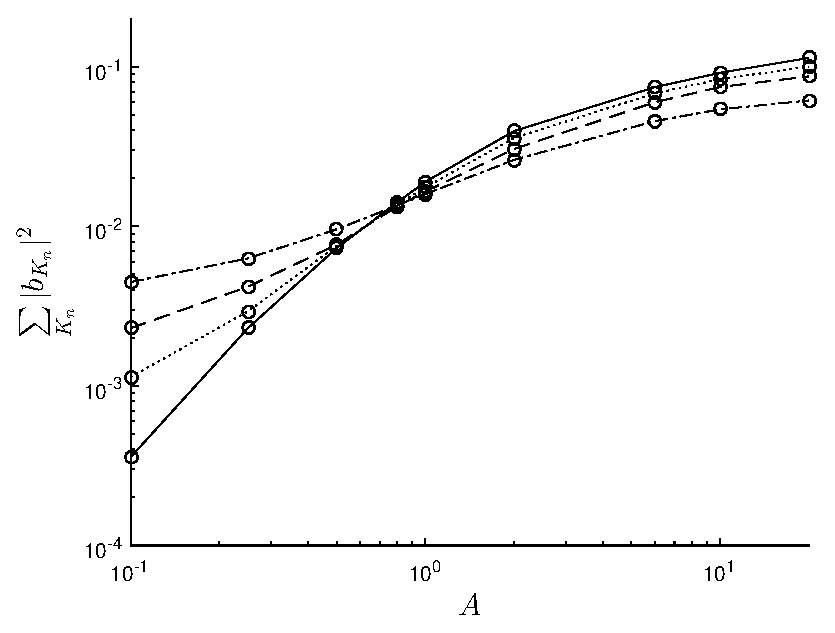
\includegraphics[width=1\linewidth]{part5/1370_fin.eps}
\captionstyle{normal}
\caption{Зависимость среднего квадрата нормированного насыщающего магнитного поля (см. (\ref{eq19plus1}))  от параметра анизотропии $A$ для продакт-бикаппа{\PunctumKappa}распределения (\ref{productkappa}) при $\beta_\perp=0.1$ и различных значениях параметра каппа: $\kappa=1$~--- штрихпунктир, $\kappa=2$~--- штрихи, $\kappa=4$~--- пунктир, $\kappa=\infty$~--- сплошная кривая (бимаксвелловское распределение).}
\label{fig:pr_kappa_sat}
\end{figure}

Проведенные нами одномерные расчеты по уравнениям (\ref{eq14})-(\ref{eq:operator}) для набора гармоник с нулевой проекцией волнового вектора на ось $y$ при $A \gg 1$ хотя и не являются вполне корректными, но дают тот же порядок величины турбулентного магнитного поля, ортогонального направлению наибольшей температуры, вдоль которого преимущественно возбуждаются вейбелевские токи и направлено электрическое поле (TM-волна в этом вырожденном случае становится обыкновенной). Сказанное согласуется с результатами давно проведенных одномерных PIC-расчетов 1D3V с осью неоднородности, параллельной оси анизотропии, вдоль которой температура минимальна; см, например,~\cite{Lemons1979,Stockem2010,Seough2015} и указанную там литературу. 
Для малых параметров анизотропии $A \ll 1$ одномерные расчеты, как и приближенная квазилинейная теория (ср.~\cite{Pokhotelov2011, Dieckmann2009, Ruyer2015}), многократно занижают насыщающее магнитное поле и неприменимы для оценки его реальных значений в двумерной и трехмерной постановках задачи. При этом критерии насыщения, по-видимому, могут быть весьма чувствительны к виду ФР и геометрии задачи, определяющим типы неустойчивости, причем как ТМ- (для необыкновенной волны), так и ТЕ- (для обыкновенной волны) типы могут развиваться одновременно. Сравнительный анализ различных качественных критериев насыщения вейбелевской неустойчивости выходит за рамки настоящей работы; они обсуждаются, например, в работах~\cite{Kocharovsky2016, Kato2005, Stockem2009,Stockem2010,YOON2011}.

Недостатком метода частиц в ячейках, кроме больших затрат вычислительных ресурсов, является высокий уровень численных шумов ФР частиц, вообще говоря, спектрально неравномерный. Это обстоятельство понижает точность и ограничивает возможность проведения корректных расчетов, особенно при малых параметрах анизотропии $A \ll 1$, когда ТМ- и ТЕ-неустойчивости развиваются настолько медленно, что скорость изотропизации частиц на шумовой компоненте электромагнитного поля становится сравнимой с инкрементом вейбелевской неустойчивости. Такого недостатка нет в развитом методе возмущений на основе пространственных гармоник, где шумы легко контролируются и могут быть адекватно заданы выбором подходящего спектра начального магнитного поля. Вместе с тем достоинством метода частиц в ячейках является кинетический учет всех трех компонент скорости частиц в двумерных (2D3V) и даже одномерных (1D3V) расчетах, отсутствующий в развитом здесь методе. Наконец, методом частиц в ячейках можно одновременно рассчитывать ТМ- и ТЕ-неустойчивости вейбелевского типа и другие кинетические неустойчивости, например пучковую для ленгмюровских волн. Таким образом, результаты расчетов согласно двум сравниваемым подходам вне рамок рассматриваемой рафинированной двумерной задачи о ТМ-турбулентности могут заметно различаться.


\subsection{Бимаксвелловское и бикаппа{\PunctumKappa}распределения}

Согласно проведенным расчетам с использованием уравнений (\ref{eq14})--(\ref{eq:operator}), для бимаксвелловского распределения средний квадрат насыщающего магнитного поля ТМ-вейбелевской неустойчивости $b_{sat}^2$ лишь немного, не более чем на 30\% превышает его значение для бикаппа{\PunctumKappa}распределений при $\kappa\geq2$; см. рис. \ref{fig:kappa_sat}. Более того, для этих бикаппа- и бимаксвелловского распределений характерные волновые числа $k_x$, отвечающие максимуму спектра развивающейся турбулентности в ортогональном оси анизотропии направлении $\vec{x_0}$, и характерные ширины этого спектра вдоль осей $x$ и $y$ оказались почти идентичными как на линейной стадии неустойчивости, так и в течении ее долговременной квазилинейной эволюции. Близость значений насыщающего магнитного поля для указанных распределений (\ref{eq:kappa}) и (\ref{bimax}) согласуется с близостью инкрементов обусловленных ими вейбелевских неустойчивостей (рис. \ref{fig:kappa_inkr}), найденных из численных расчетов среднеквадратичного магнитного поля на этапе его экспоненциального роста задолго до момента насыщения. Эти инкременты лишь немного меньше максимальных инкрементов, вычисленных из соответствующих дисперсионных уравнений (о последних см., например,~\cite{Mikhailovsky1971, Lazar2006, Vagin2014, Kocharovsky2016,Ruyer2015,Silva2021}). 
\begin{figure}[h]

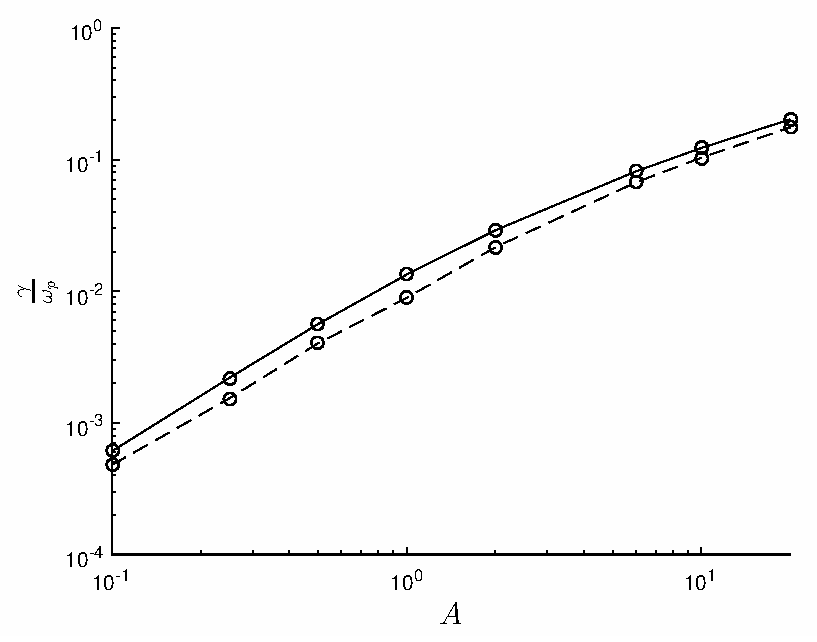
\includegraphics[width=1\linewidth]{part5/kappa_inkr.eps}
\captionstyle{normal}
\caption{Зависимость инкремента $\gamma$ (нормированного на плазменную частоту $\wpl$) среднеквадратичного магнитного поля от параметра анизотропии $A$ для бикаппа{\PunctumKappa}распределения (\ref{eq:kappa}) при $\beta_\perp=0.1$ и различных значениях параметра каппа: $\kappa=2$~--- штрихи, $\kappa=\infty$~--- сплошная кривая (бимаксвелловское распределение).}
\label{fig:kappa_inkr}
\end{figure}

Полученный результат согласуется также с практически одинаковой формой деформации указанных ФР электронов к моменту насыщения неустойчивости, о чем можно судить, прежде всего, из найденных в наших расчетах пространственно однородных поправок $\delta f_0(v_x, v_y)$, т.\,е. $\psi_0(\beta_x, \beta_y)$. Соответствующая деформация ФР вызвана совокупным действием всех гармоник квазимагнитостатической турбулентности и в свою очередь определяет квазилинейную эволюцию каждой из этих гармоник, непосредственно не взаимодействующих между собой: их начальное нарастание, длительное существование с медленным изменением амплитуды и последующее неизбежное затухание. Более подробный анализ данного круга явлений, изученных нами численно, заслуживает отдельной публикации и может позволить продвинуться в аналитическом описании двумерной ТМ-турбулентности после ее насыщения, а также дополнить имеющуюся квазилинейную теорию одномерной вейбелевской неустойчивости при малых значениях параметра анизотропии $A$~\cite{Pokhotelov2011}. 

ё1



\subsection{Продакт-бикаппа{\PunctumKappa}распределение}

Детализируем сделанные выше общие утверждения применительно к продакт- бикаппа{\PunctumKappa}распределению (\ref{productkappa}), для которого обнаруживается существенное влияние величины $\kappa$ на исследуемую зависимость насыщающего поля от начальной анизотропии ФР, особенно в области ее малых величин $A<0.8$ согласно рис.~\ref{fig:pr_kappa_sat}. Монотонные зависимости среднего квадрата насыщающего магнитного поля от параметра анизотропии $A$ для различных величин $\kappa$ имеют разный наклон и пересекаются в одной точке $A=0.8$. При $A \sim 0.1$ эти зависимости приближенно являются степенными с показателями, которые примерно равны 2/5, 2/3, 1, 2 для $\kappa =$ 1, 2, 4, $\infty$ соответственно (и могут оказаться меньше при $A < 0.1$).  

Ниже точки $A=0.8$ квадрат насыщающего магнитного поля $b_{sat}^2$ значительно падает с ростом величины $\kappa$, достигая минимального значения при $\kappa \rightarrow \infty$, т.\,е. для бимаксвелловского распределения. Напротив, выше указанной точки $A=0.8$ величина $b_{sat}^2$ растет с ростом $\kappa$, хотя и не столь значительно, поскольку ее максимальное значение для величины $\kappa$ вблизи 1 составляет несколько процентов и всего в пару раз меньше предельно достижимого значения квадрата магнитного поля $b_{sat}^2$, реализующегося для бимаксвелловского распределения и немного превышающего 10\%. 

Для продакт-бикаппа{\PunctumKappa}распределений в отличие от бикаппа{\PunctumKappa}распределений величина $\kappa$ гораздо значительнее влияет на нелинейную эволюцию как характерного волнового числа $k_x$, отвечающего максимуму спектра турбулентности и направленного в ортогональном оси анизотропии направлении $\vec{x_0}$, так и характерных ширин турбулентного спектра вдоль осей $x$ и $y$. С ростом величины $\kappa$ уширение спектра вдоль оси анизотропии ФР увеличивается, тогда как ширина спектра поперек этой оси уменьшается одновременно с уменьшением указанной проекции $k_x$ волнового вектора максимума турбулентного спектра. Подобное уменьшение наиболее существенно на начальной нелинейной стадии эволюции спектра (и становится довольно малым на поздней стадии, которой мы не интересуемся в настоящей работе).

Сделанное наблюдение согласуется с уменьшением при росте $\kappa$ инкремента нарастания магнитного поля (рис.~\ref{fig:pr_kappa_inkr}), вычисленного на линейной стадии задолго до насыщения неустойчивости и примерно равного максимальному инкременту, получающемуся из соответствующего дисперсионного уравнения (см.~о~нем~\cite{Mikhailovsky1971, Lazar2006, Vagin2014, Kocharovsky2016,Ruyer2015,Silva2021}). Уменьшение инкремента с увеличением $\kappa$ от 1 до $\infty$ значительно лишь для небольшой начальной анизотропии $A \lesssim 1$: для $A=1$ инкремент уменьшается примерно вдвое, а для $A=0.1$~--- в 20 раз. Заметим, что в последнем случае почти в 20 раз уменьшается и квадрат насыщающего магнитного поля $b_{sat}^2$ (рис.~\ref{fig:pr_kappa_sat}). Вместе с тем это поле слабо зависит от величины $\kappa$ при большой начальной анизотропии $A \gg 1$.
\begin{figure}[h]
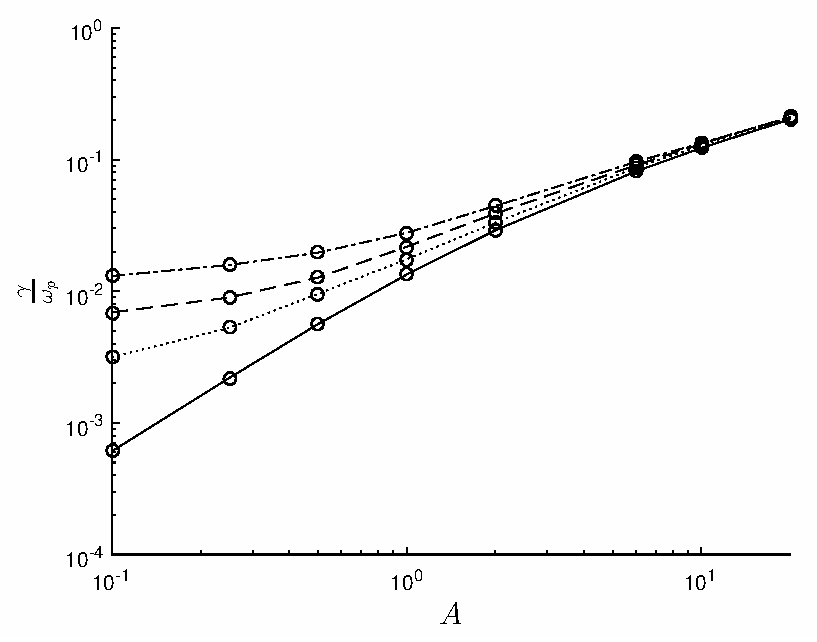
\includegraphics[width=1\linewidth]{part5/1372_fin.eps}
\captionstyle{normal}
\caption{Зависимость инкремента $\gamma$ (нормированного на плазменную частоту $\wpl$) среднеквадратичного магнитного поля от параметра анизотропии $A$ для продакт-бикаппа{\PunctumKappa}распределения (\ref{productkappa}) при $\beta_\perp=0.1$ и различных значениях параметра каппа: $\kappa=1$~--- штрихпунктир, $\kappa=2$~--- штрихи, $\kappa=4$~--- пунктир, $\kappa=\infty$~--- сплошная кривая (бимаксвелловское распределение).}
\label{fig:pr_kappa_inkr}
\end{figure}
Выведенная в настоящей работе система приближенных уравнений (\ref{eq14})--(\ref{eq19}), (\ref{eq:operator}) для ТМ-гармоник турбулентности позволяет исследовать  насыщение вейбелевской неустойчивости и ее дальнейшую нелинейную эволюцию при малых величинах параметра анизотропии, включая область $A \lesssim 0.01$ (которая вряд ли легко доступна расчетам методом частиц в ячейках из-за неизбежных для него численных шумов). Подобная близость к порогу неустойчивости характерна для многих физических ситуаций, и особенности обсуждаемого эффекта насыщения роста ТМ-вейбелевской турбулентности в этих условиях заслуживают специального исследования.


В случае ТЕ-вейбелевской неустойчивости для волн обыкновенного типа~\cite{Mikhailovsky1971, Gary1993, Vagin2014, Kocharovsky2016, Rubab2016}, когда вектор электрического поля возмущения ортогонален плоскости, образованной волновым вектором возмущения и осью анизотропии ФР, аналогичные детальные расчеты насыщающего магнитного поля для тех или иных бикаппа{\PunctumKappa}распределений, включая бимаксвелловское, еще не проводились. Эта задача представляет интерес, поскольку в определенных условиях, например, для ФР в форме сплюснутого эллипсода или диска, значение инкремента ТЕ-вейбелевской неустойчивости может превышать его значение для одновременно развивающейся ТМ-неустойчивости. Вследствие многобразия и неопределенности параметров ФР, ожидаемых в различных условиях, даже для линейной стадии неустойчивости отсутствует сколько-нибудь полная картина зависимости максимальных ТЕ- и ТМ-инкрементов и соответствующих им оптимальных волновых чисел от параметра анизотропии $A$; ср., например,~\cite{Lazar2010, Zaheer2007, Rubab2016, YOON2011, Silva2021}. Имея в виду трудоемкость расчетов, подобную зависимость, как и аналогичную зависимость насыщающего магнитного поля, а тем более характера долговременной нелинейной эволюции вейбелевской турбулентности следует изучать для конкретного типа ФР в неравновесной плазме.

В этом отношении актуальны, например, задачи лабораторной астрофизики с лазерной плазмой~\cite{Romanov2004, Thaury2010, Silva2020, Shukla2020, Zhang2020}, получаемой абляцией различных мишеней фемтосекундными импульсами петаваттных лазеров, и задачи физики солнечного (звездного) ветра, начиная с корональных областей его происхождения и кончая границами между магнитными облаками в нем или областями его взаимодействия с магнитосферами планет~\cite{Baumjohann2012, Dudik2017, Livadiotis2017,Marsch2006,Yoon2017,Echim2010}. Для обоих указанных классов задач имеется непосредственная возможность получать информацию как о распределении частиц по энергии, так и об анизотропии распределения частиц по скоростям. Наблюдаемое наличие надтеплового {\glqq}хвоста{\grqq} в энергетическом распределении частиц~\cite{Maksimovic2005, Vasyliunas1968,Lazar2022}, свойственное различным каппа{\PunctumKappa}распределениям, делает последние удобными для использования в численном моделировании процессов развития вейбелевской неустойчивости и генерации долгоживущей квазимагнитостатической турбулентности. 

Начатое в настоящей работе исследование зависимостей насыщающего среднеквадратичного магнитного поля от параметров каппа $\kappa$ и анизотропии $A$ представляется важным для оценки влияния такого рода турбулентности на ряд наблюдаемых явлений в лазерной и космической плазме. В частности, важными представляются найденные конкретные зависимости уровня насыщения вейбелевской турбулентности от параметра анизотропии, которые для одних ФР (например, бикаппа{\PunctumKappa} и бимаксвелловской) оказываются близкими, а для других (продакт-бикаппа-распределений с разными значениями $\kappa$)~--- сильно различающимися при $A < 0.3$.

Полученная и использованная нами система уравнений для взаимодействующих гармоник возмущений магнитного поля и ФР особенно перспективна для анализа эволюции квазимагнитостатической турбулентности в случае малой анизотропии ФР, т.\,е. при небольшом превышении порога вейбелевской неустойчивости, что является типичным, в частности, для плазмы солнечного ветра, а также для лазерной плазмы после прекращения подкачки в нее энергичных электронов. Более того, эта система уравнений применима и для описания развития неустойчивости даже в отсутствие анизотропии эффективных температур немаксвелловской ФР, когда профиль энергетического распределения частиц играет определяющую роль~\cite{Silva2021,Lazar2010}. Для подобных задач преимущества расчета на основе предложенной системы уравнений по сравнению с обычным расчетом методом частиц в ячейках могут оказаться важными.

Кроме продолжения исследований в указанном направлении, в отдельной статье предполагается представить результаты исследования обнаруженного нами сильного влияния на ТМ-турбулентность внешнего крупномасштабного магнитного поля, ориентированного вдоль оси анизотропии ФР. Такое поле зачастую присутствует в космической плазме, в том числе в солнечном ветре, а на лазерную плазму может быть наложено извне, в частности, с целью проведения экспериментов по широко развивающейся лабораторной астрофизике. Как и в исследованной выше задаче, в этих условиях ожидается существенная роль анизотропии пространственного спектра развивающейся мелкомасштабной квазимагнитостатической турбулентности, способной значительно изменить крупномасштабную структуру полного магнитного поля, а следовательно, и динамику неравновесной плазмы в нем. Естественно, в каждой конкретной ситуации необходимо сравнивать неустойчивость вейбелевского типа с другими возможными неустойчивостями анизотропной плазмы, особенно апериодическими~\cite{Lazar2022,Shaaban2021,Shaaban2019,Yoon2017,Dieckmann2019,StockemNovo2015}, которые могут конкурировать в создании той или иной магнитной турбулентности. Подобный сравнительный анализ представляется весьма актуальным.
















